
\chapter{Introduction}\label{chapter:introduction}
%Breast cancer bad 
Breast cancer is the most common form of cancer diagnosed worldwide
and the leading cause of cancer-related death among women~\cite{chhikara2022global}.
It is a heterogeneous disease, consisting of several morphological and molecular subtypes.
The molecular subtypes are among the prime factors to characterize breast cancer.
There are four common clinically relevant subtypes~\cite{home} defined on the status of three receptors,
namely the Hormonal Receptor (HR, which is positive if either Estrogen Receptor (ER)
or Progesterone Receptor (PR) is positive) and the human epidermal
growth factor receptor 2 (Her2):
\begin{enumerate}
    \itemsep0em 
    \item Luminal A (HR positive, Her2 negative)
    \item Luminal B (HR positive, Her2 positive)
    \item Her2 enriched (HR negative, Her2 positive) 
    \item Triple Negative (HR negative, Her2 negative)
\end{enumerate}
Regardless of the subtype, breast cancer is primarily classified by its histological appearance. 
Thus for diagnostic confirmation, a patient’s biopsy or surgical resection samples
are sectioned onto microscope slides for staining, often with hematoxylin and eosin
(H\&E), followed by a visual diagnosis by a pathologist. Pathologists examine the
tissue for abnormalities that indicate breast cancer. 
Cancer causes changes in the tissue at the sub-cellular scale, hence an analysis of normal
and tumor tissue can provide novel insights into
tissue characteristics, lead to a better understanding of mechanisms
underlying cancer progression and provide valuable information for medical
decision-making such as tumor grading and treatment choices~\cite{vu2019methods}.

One of the characteristics of histological images that can be visually assessed by pathologists is lymphocytic infiltration.
There are a number of publications that emphasize the prognostic value of tumor-infiltrating lymphocytes (TILs),
especially in triple negative (TNBC) and human epidermal growth factor receptor 2 (HER2+) breast cancer~\cite*{salgado2015evaluation, denkert2018tumour}.
TILs are mononuclear immune cells that infiltrate tumor tissue.
They have been detected in almost all solid tumors, including breast cancer~\cite{laenkholm2022incorporation}.
The development and progression of malignant tumors can be characterized by an interaction between the cells
in the tumor microenvironment and TILs.
In the early stage of HER2+ and TNBC, TILs are detectable in up to 75\% of tumors~\cite{dieci2018update}.
Studies have shown that an increased degree of lymphocytic infiltration is predictive of better
long-term control of the disease~\cite{adams2014prognostic, loi2013prognostic}.
Patients with a high proportion of TILs in the tumor tissue and high immunogenicity of the tumor were shown
to respond better to chemotherapy~\cite{denkert2010tumor}.
Accumulating evidence indicates that tumor-infiltrating lymphocytes are clinically useful biomarkers
in TNBC and HER2+ and that they play an essential role in cancer progression~\cite{gao2020prognostic}.
Further research and development of TIL related biomarkers would grant clinicians
essential prognostic information and promote the research on novel treatments and therapeutics.
For instance, since TILs with exhausted phenotype are associated with loss of antitumor immunity,
single-cell RNA Sequencing of TILs has been already performed to search for new immune checkpoint blockade
targets that enable the precise definition and even novel development of therapeutic strategies to overcome T-cell exhaustion.
Therapeutic approaches to influence T-cell exhaustion have been developed to target proteins CTLA-4,
PD-1, and PD-L1 and have proven to be effective in treating melanoma and non-small-cell lung cancer
during ongoing trials~\cite{postow2015immune}.
TILs in TNBC patients also display immuno-suppressive phenotypes~\cite{chung2017single} and the number
of TILs detected by TNBC patients is one of the highest of all breast cancer subgroups~\cite{schneeweiss2019diagnosis}
which makes TNBC a valid target for further TILs research.

A valuable contribution to TILs research and any task involving visual analysis
of histological images would be method automatization.
While manual examination continues to be widely applied in a clinical setting,
it is subjective and not scalable to translational and clinical research studies
involving large datasets of high-resolution whole slide tissue images (WSIs).
Hence, there is a raised demand for reliable and efficient automated methods to
complement the traditional manual examination of tissue samples. 

With advancing technology and access to a large amount of data, deep learning
methods have garnered an interest in computational pathology. 
There are multiple deep learning-based methods and pipelines that have been
proposed for detection and segmentation tasks of WSIs. 
To stimulate the development of algorithms for automatic TILs evaluation,
a special Tumor InfiltratinG lymphocytes in breast cancER (TiGER)~\cite{home}
challenge was formed. Within this competition, various algorithms were
evaluated for the automated assessment of TILs in H\&E stained
histopathology WSIs that resulted in automatically acquired TILs scores.
Those were later internally checked for significance as prognostic values
and the concordnace was reported.
The clinical focus of the TiGER challenge is on Her2+ and TNBC.
It is motivated by research and clinical data that show that Her2+
and TNBC have the worst prognosis making them an intense target of
prognostic and predictive biomarker research aimed at improving patient
management and prognosis.

This work is closely linked to the TiGER challenge. The goal is to develop a pipeline
for HER2 positive and triple negative breast cancer H\&E slides
that segments tumor and stroma regions, detects TILs, and produces TILs scores
as pictured in Figure~\ref*{fig:workflow} block 1-3.
\begin{figure}[H]
    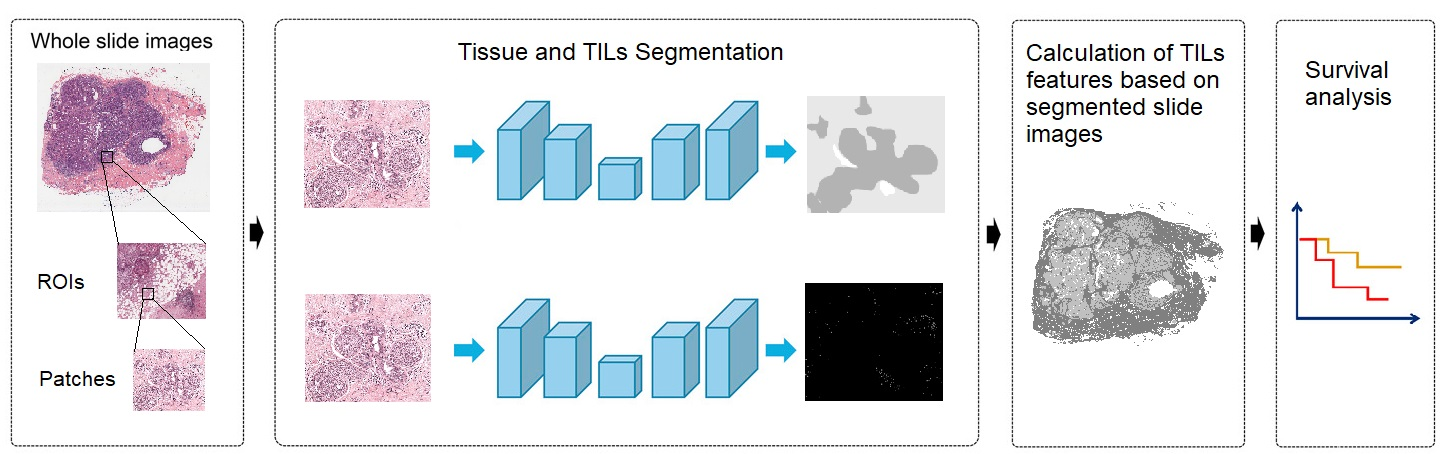
\includegraphics[width=\linewidth]{figures/overview.jpg}
    \caption{Abstract scheme to visually introduce the flow of this thesis work.}
    \label{fig:workflow}
\end{figure}
This work takes benefit of the annotated region of interests (ROIs) provided by the TiGER challenge
for the development of patch-based automated tissue and TIL segmentation.
As a step beyond the challenge, the scores based on the degree of lymphocytic
infiltration are evaluated on the breast cancer TCGA-BRCA dataset generated by
the TCGA Research Network and not on the hidden TiGER dataset which is not available
after the end of the competition.
The TCGA-BRCA clinical data enables independent broad survival analysis of different experimental
TIL characteristics that can be calculated solely based on histological images (Figure~\ref*{fig:workflow} block 4). 
As a result, this work aims not only to develop a computational approach
to compute TIL score on H\&E images of Her2+ and TNBC but also experiment
with different TIL scores and show detailed survival analysis based on publically available
TCGA-BRCA dataset together with their predictive value for overall patient survival. 
